\documentclass{article}

\usepackage{graphicx}
\usepackage{float}

\title{Applicazione per la gestione del cibo}

\date{2024-05-10}

\author{Saverio Napolitano}

\begin{document}

\maketitle

\pagenumbering{gobble}

\newpage

\pagenumbering{arabic}

\section{Introduzione}

TODO.

\section{Specifica dei requisiti}

TODO.

\subsection{Requisiti funzionali}

TODO.

\subsection{Requisiti non funzionali}

TODO.

\section{Descrizione del progetto}

TODO.

\begin{figure}[H]
    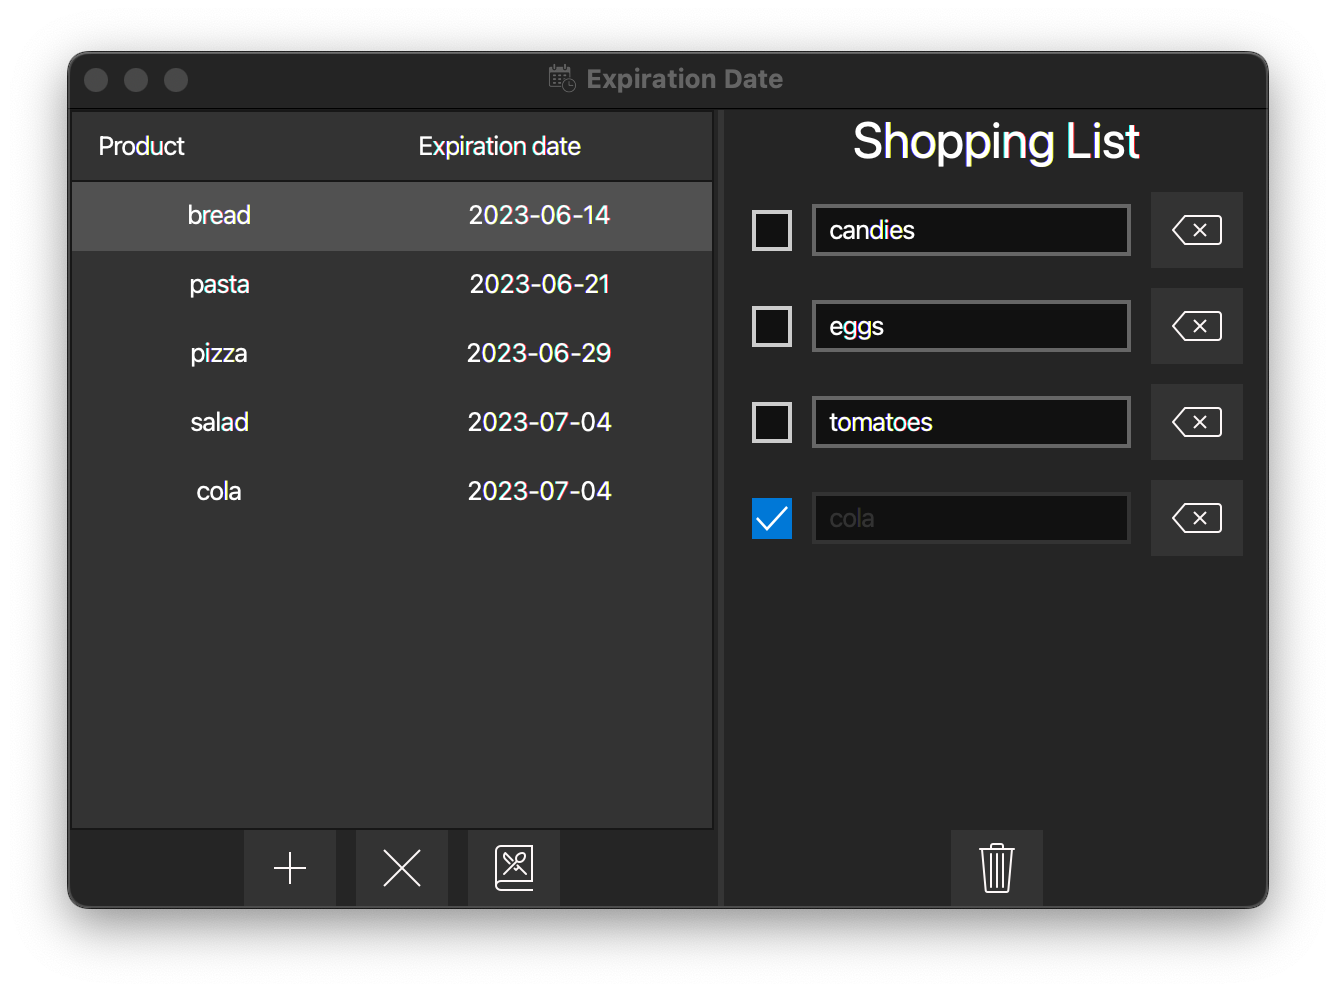
\includegraphics[width=\linewidth]{images/main-view.png}
    \caption{Finestra per la gestione di dispensa e lista della spesa.}
    \label{fig:mainview}
\end{figure}

\begin{figure}[H]
    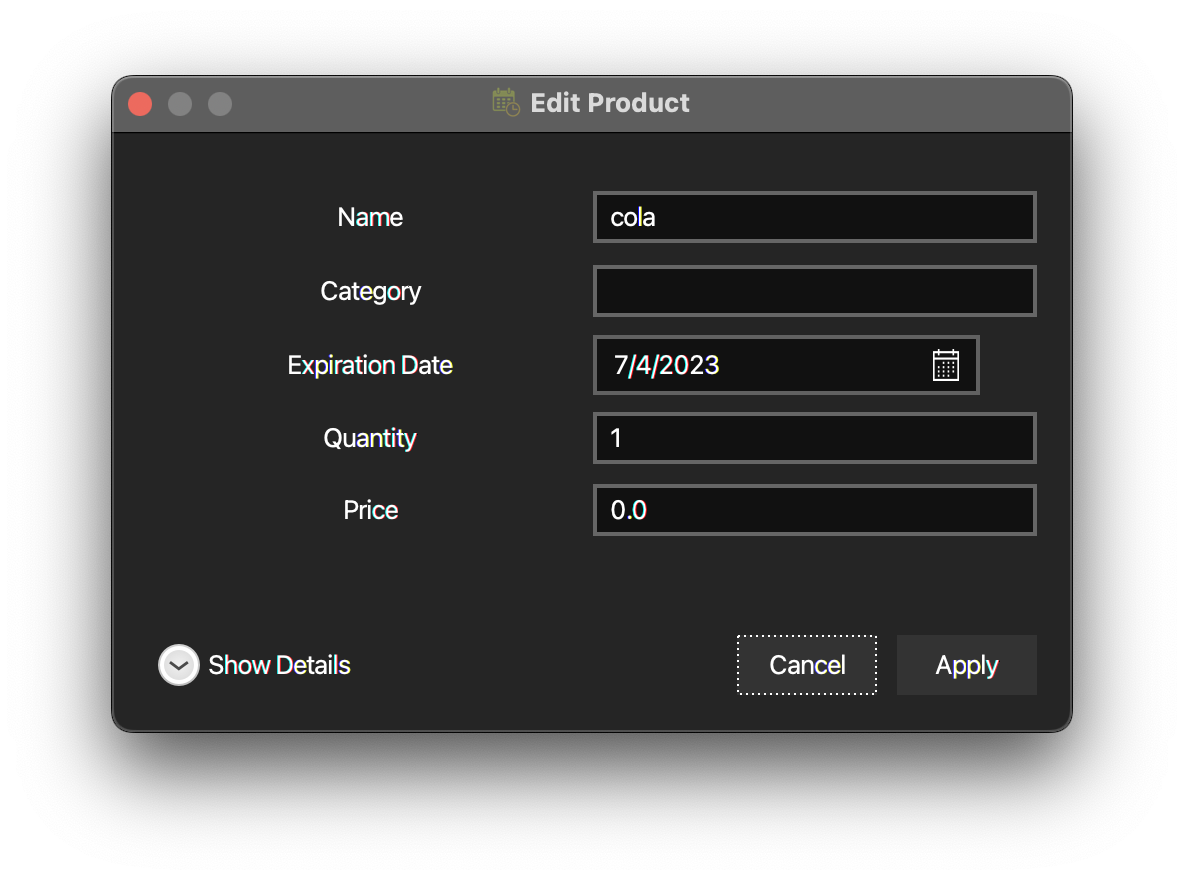
\includegraphics[width=\linewidth]{images/edit-product.png}
    \caption{Finestra per la modifica dei dati del prodotto.}
    \label{fig:editproduct}
\end{figure}

\begin{figure}[H]
    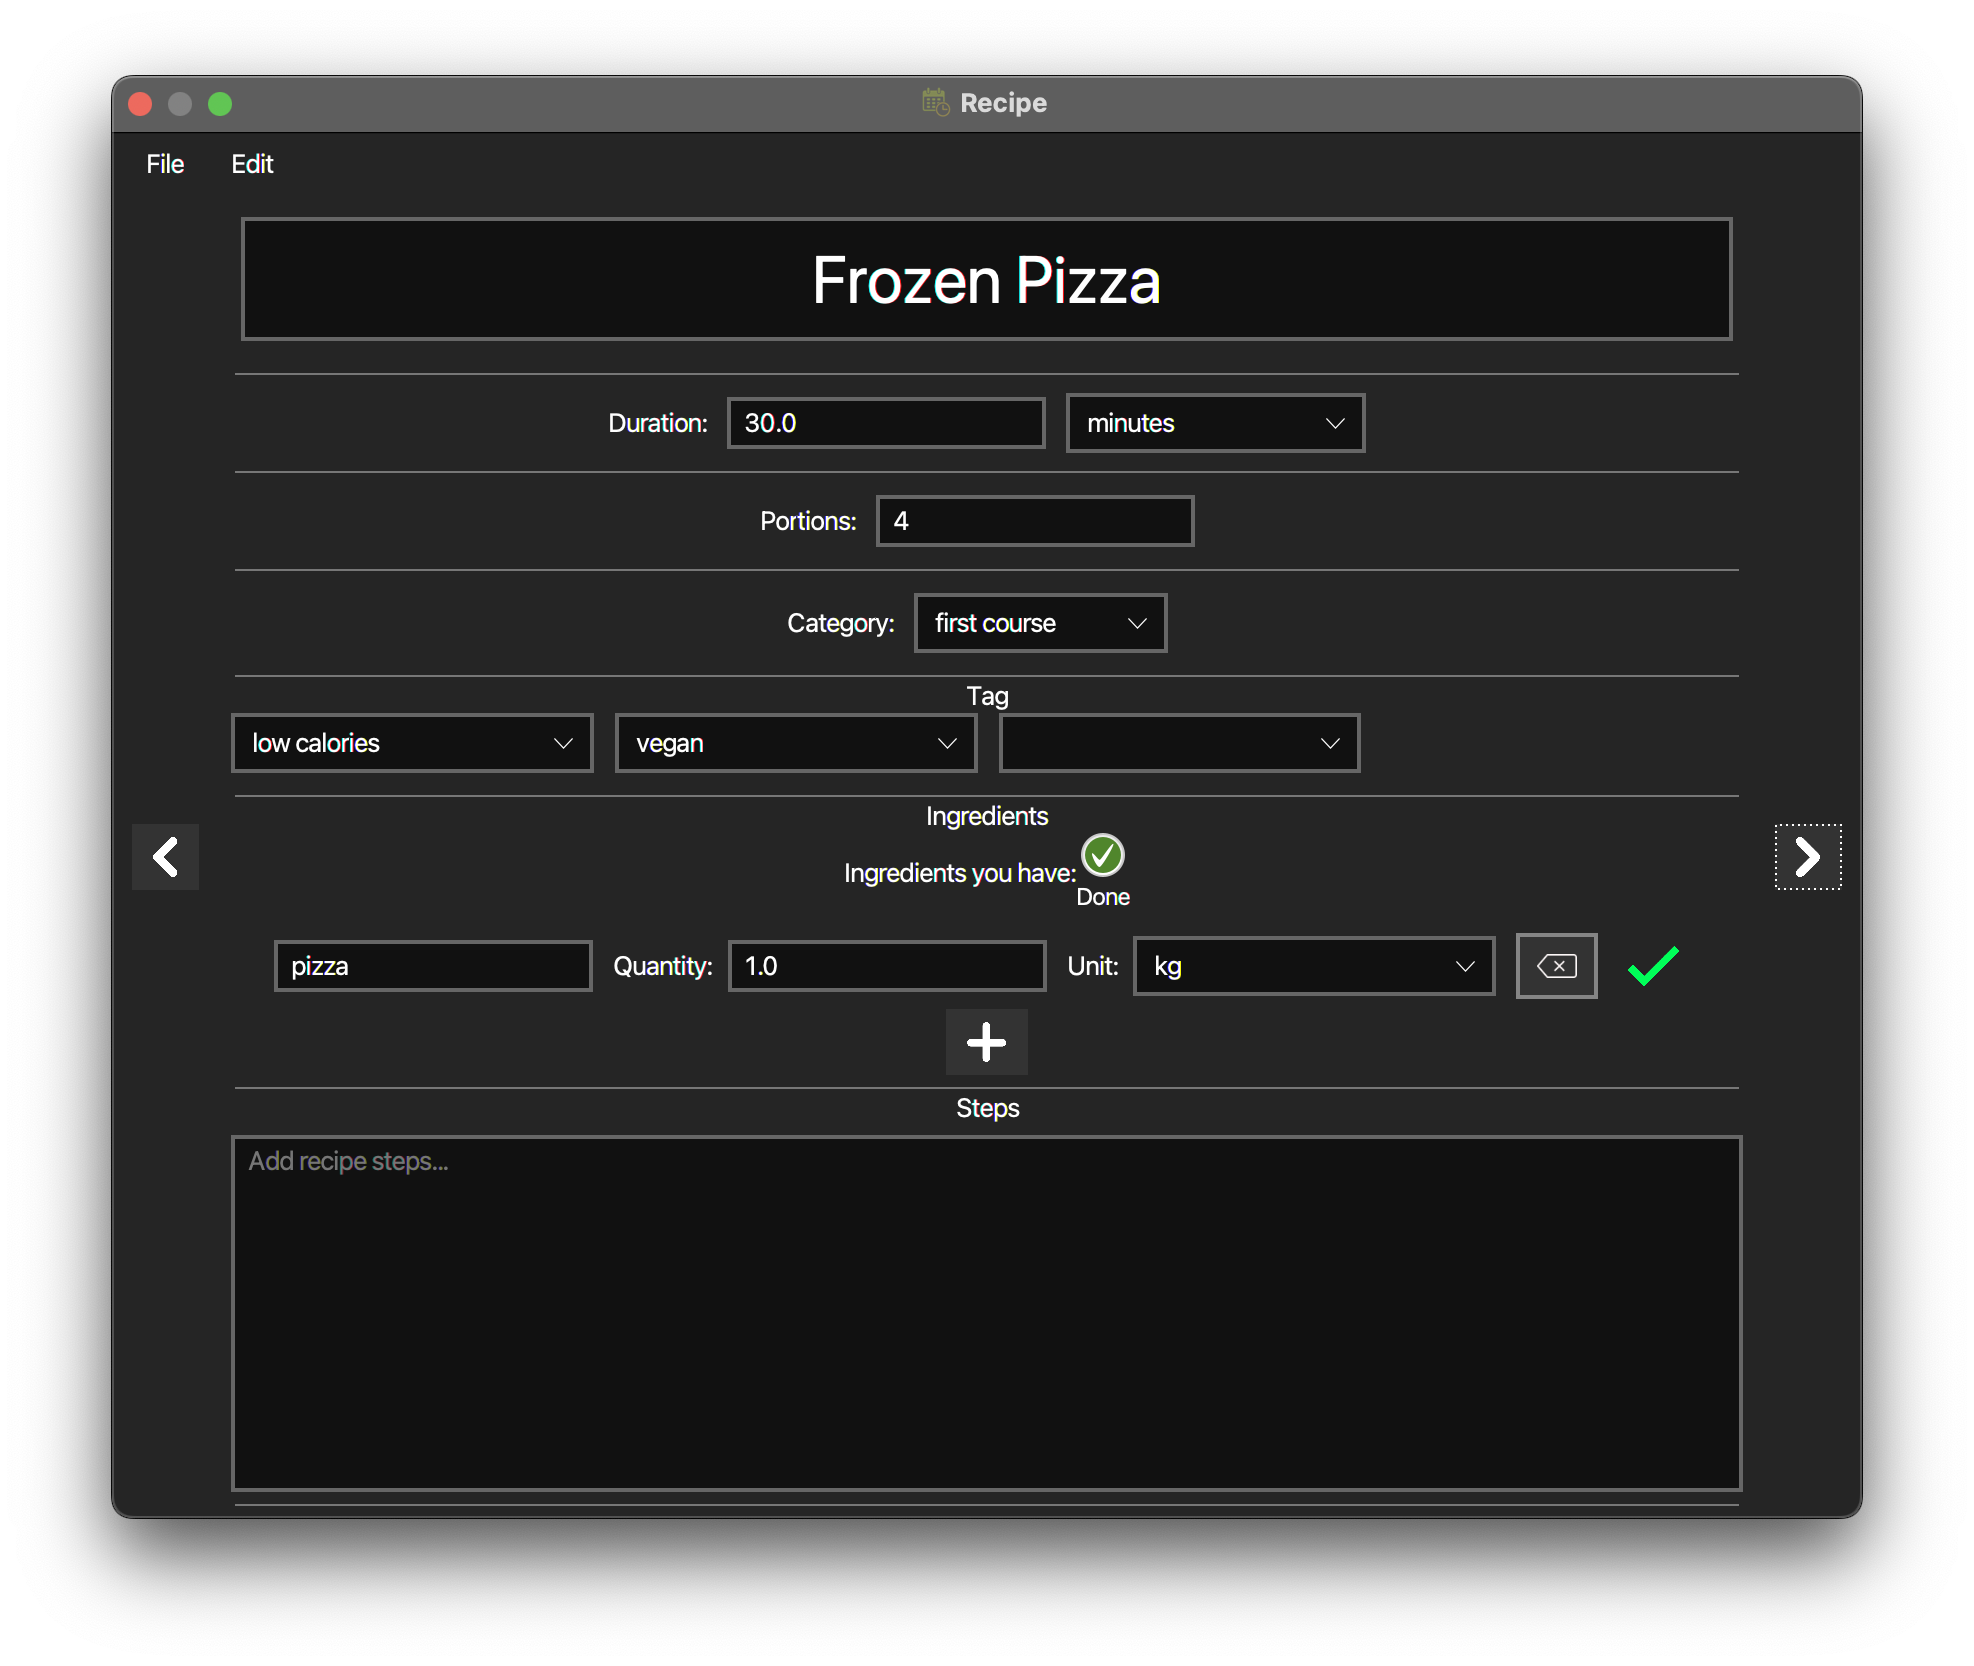
\includegraphics[width=\linewidth]{images/recipe-view.png}
    \caption{Finestra per la gestione delle ricette.}
    \label{fig:recipeview}
\end{figure}

\section{UML}

TODO.

\subsection{Use case diagram}

TODO.

\begin{figure}[h!]
    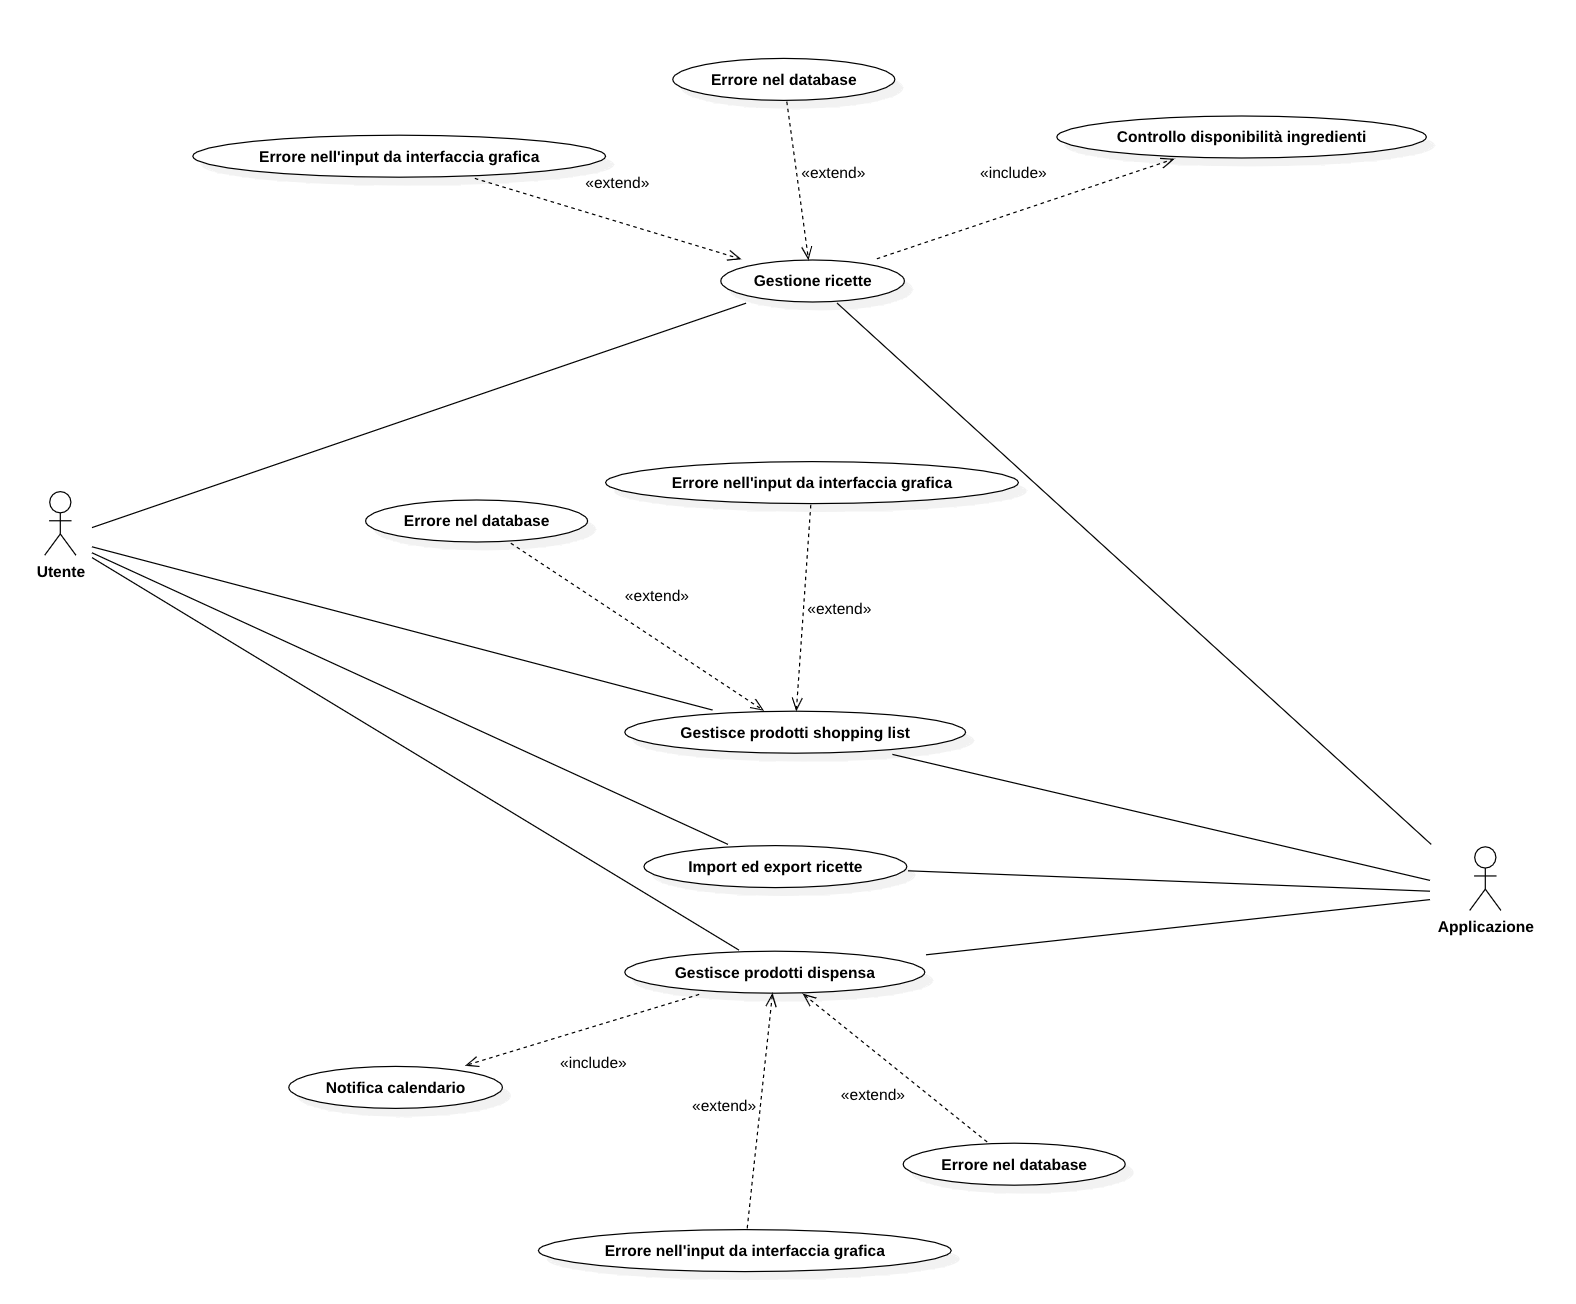
\includegraphics[width=\linewidth]{images/use-case.png}
    \caption{Diagramma dei casi d'uso.}
    \label{fig:usecase}
\end{figure}

\subsection{Activity diagram}

TODO.

\subsubsection{Activity diagram della dispensa}

TODO.

\begin{figure}[H]
    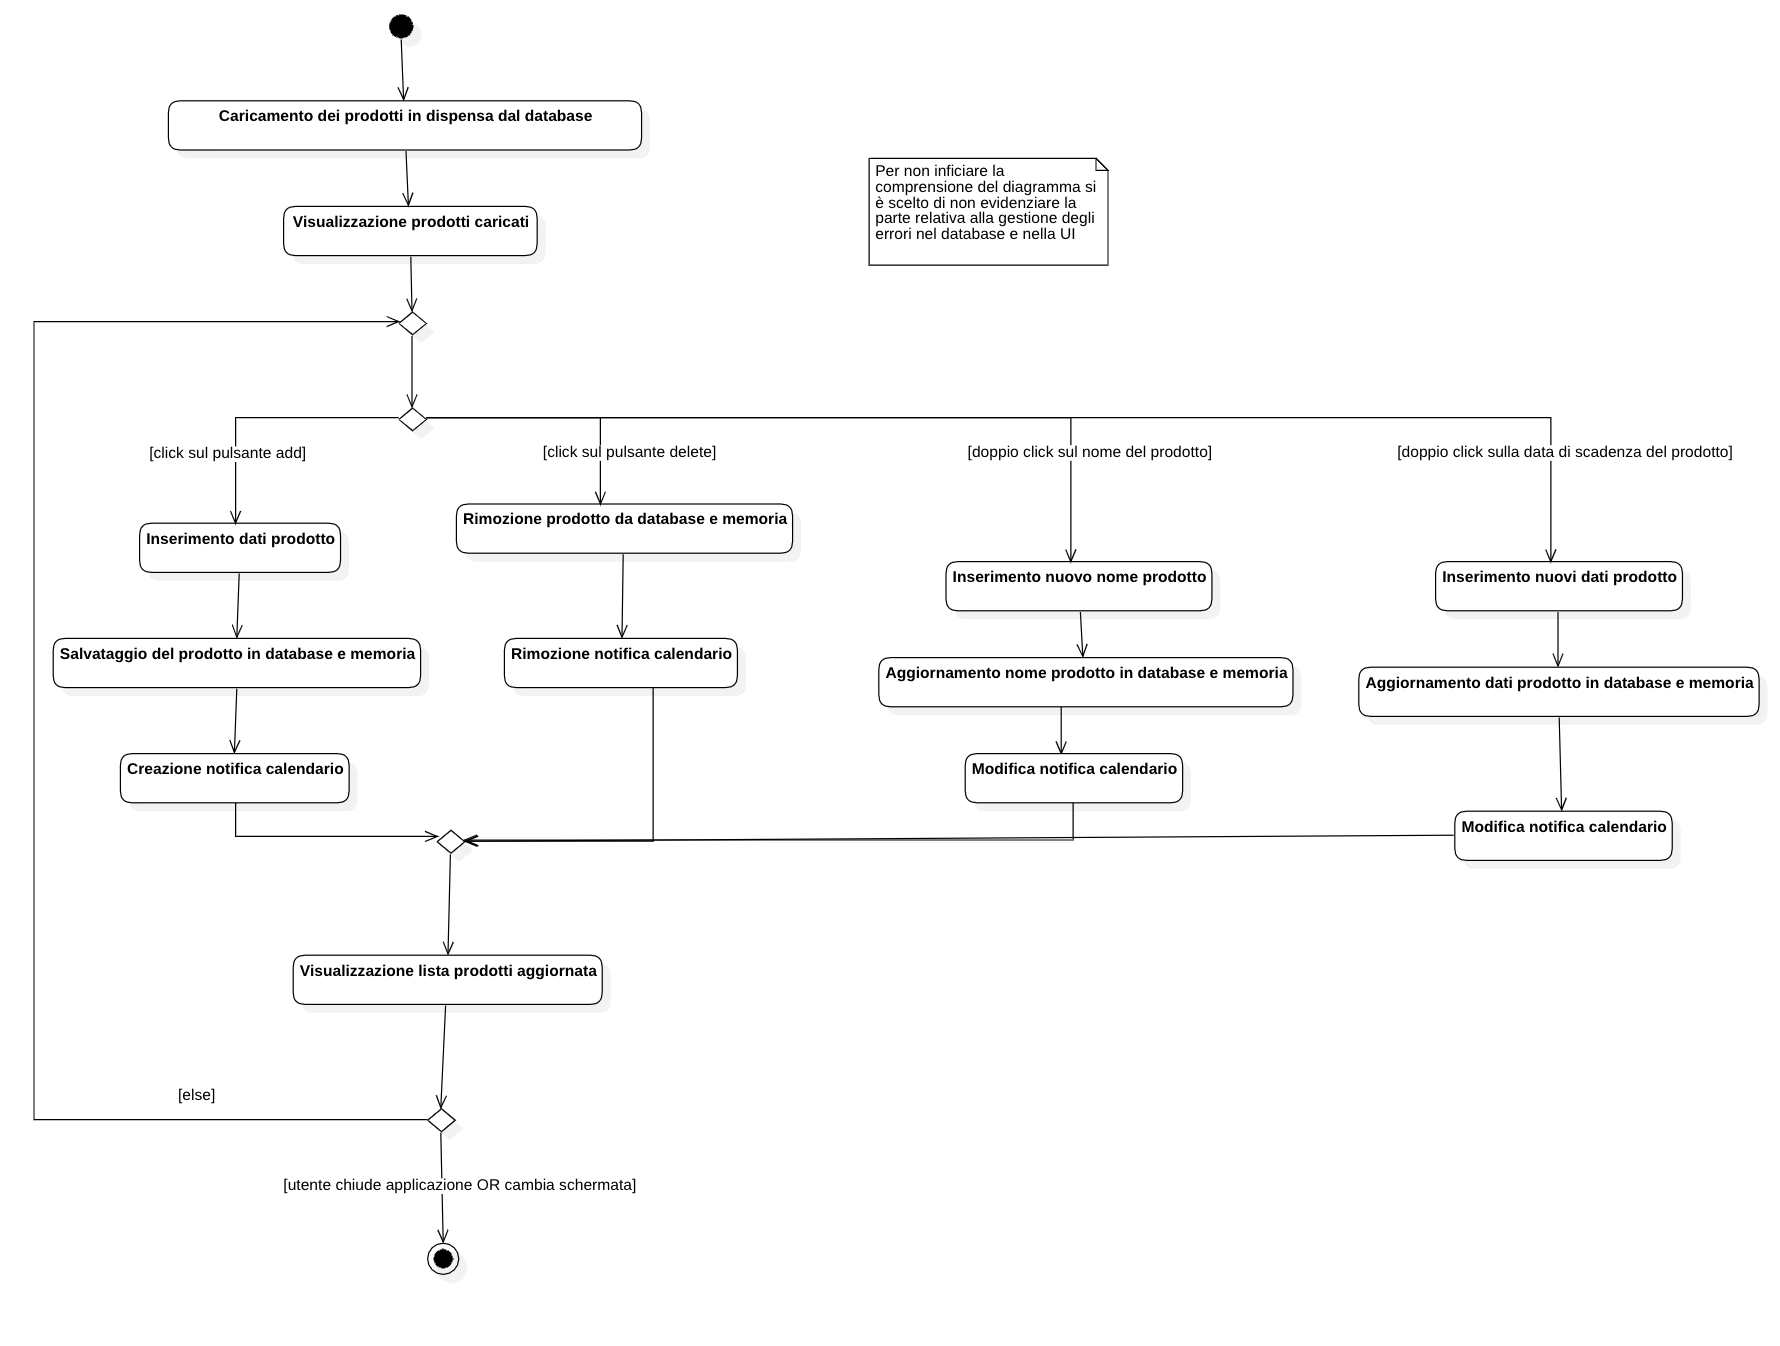
\includegraphics[width=\linewidth]{images/activity-pantry.png}
    \caption{Diagramma delle attività della dispensa.}
    \label{fig:actpantry}
\end{figure}

\subsubsection{Activity diagram della lista della spesa}

TODO.

\begin{figure}[H]
    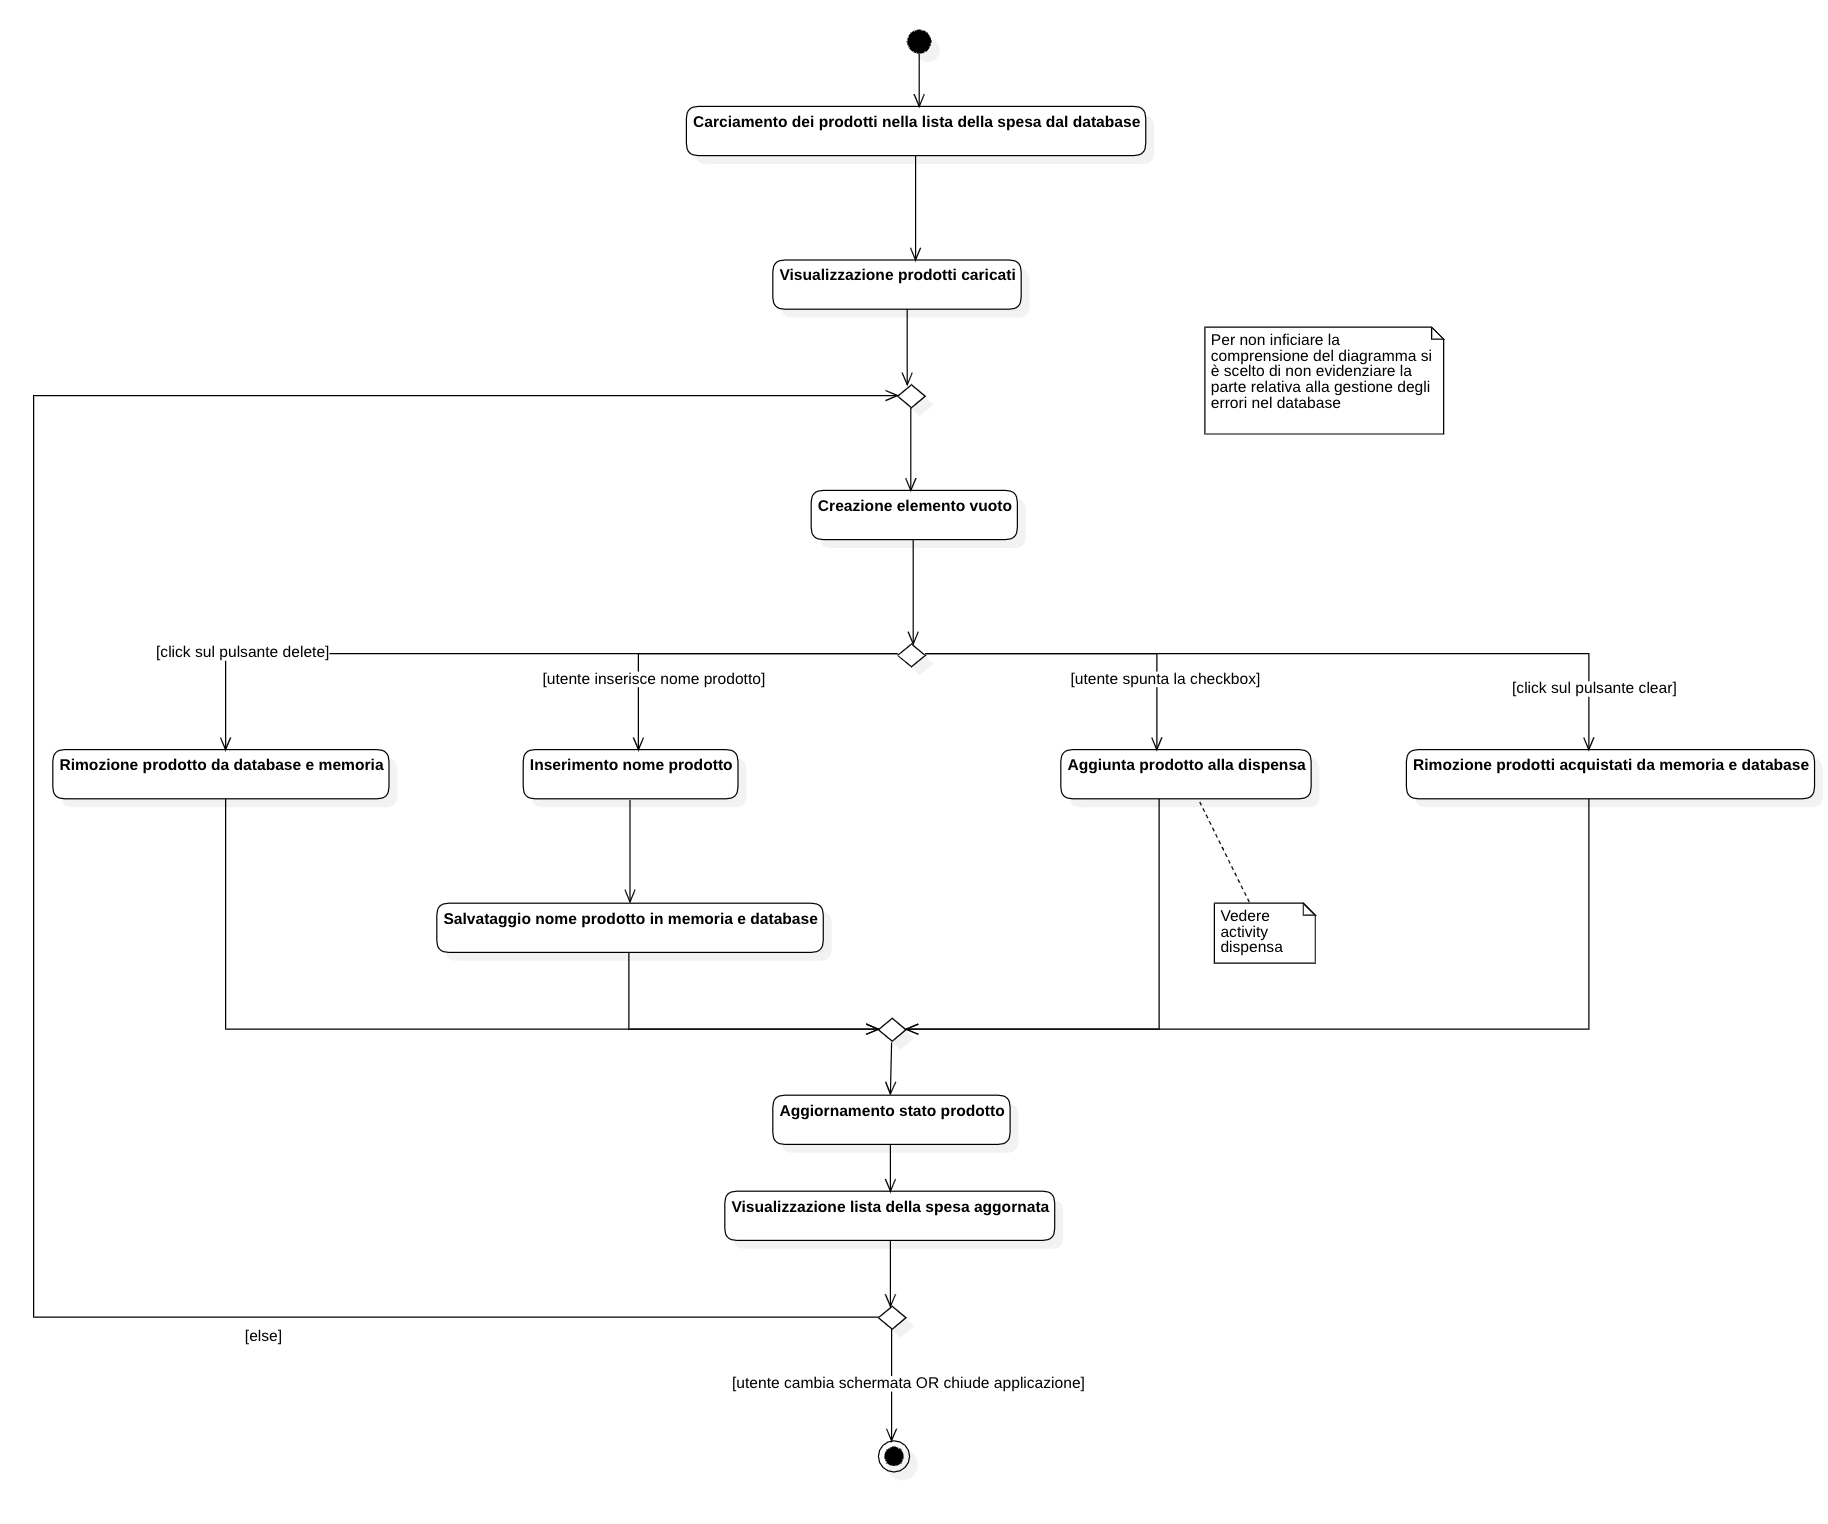
\includegraphics[width=\linewidth]{images/activity-shopping-list.png}
    \caption{Diagramma delle attività della lista della spesa.}
    \label{fig:actshoplist}
\end{figure}

\subsubsection{Activity diagram delle ricette}

TODO.

\begin{figure}[H]
    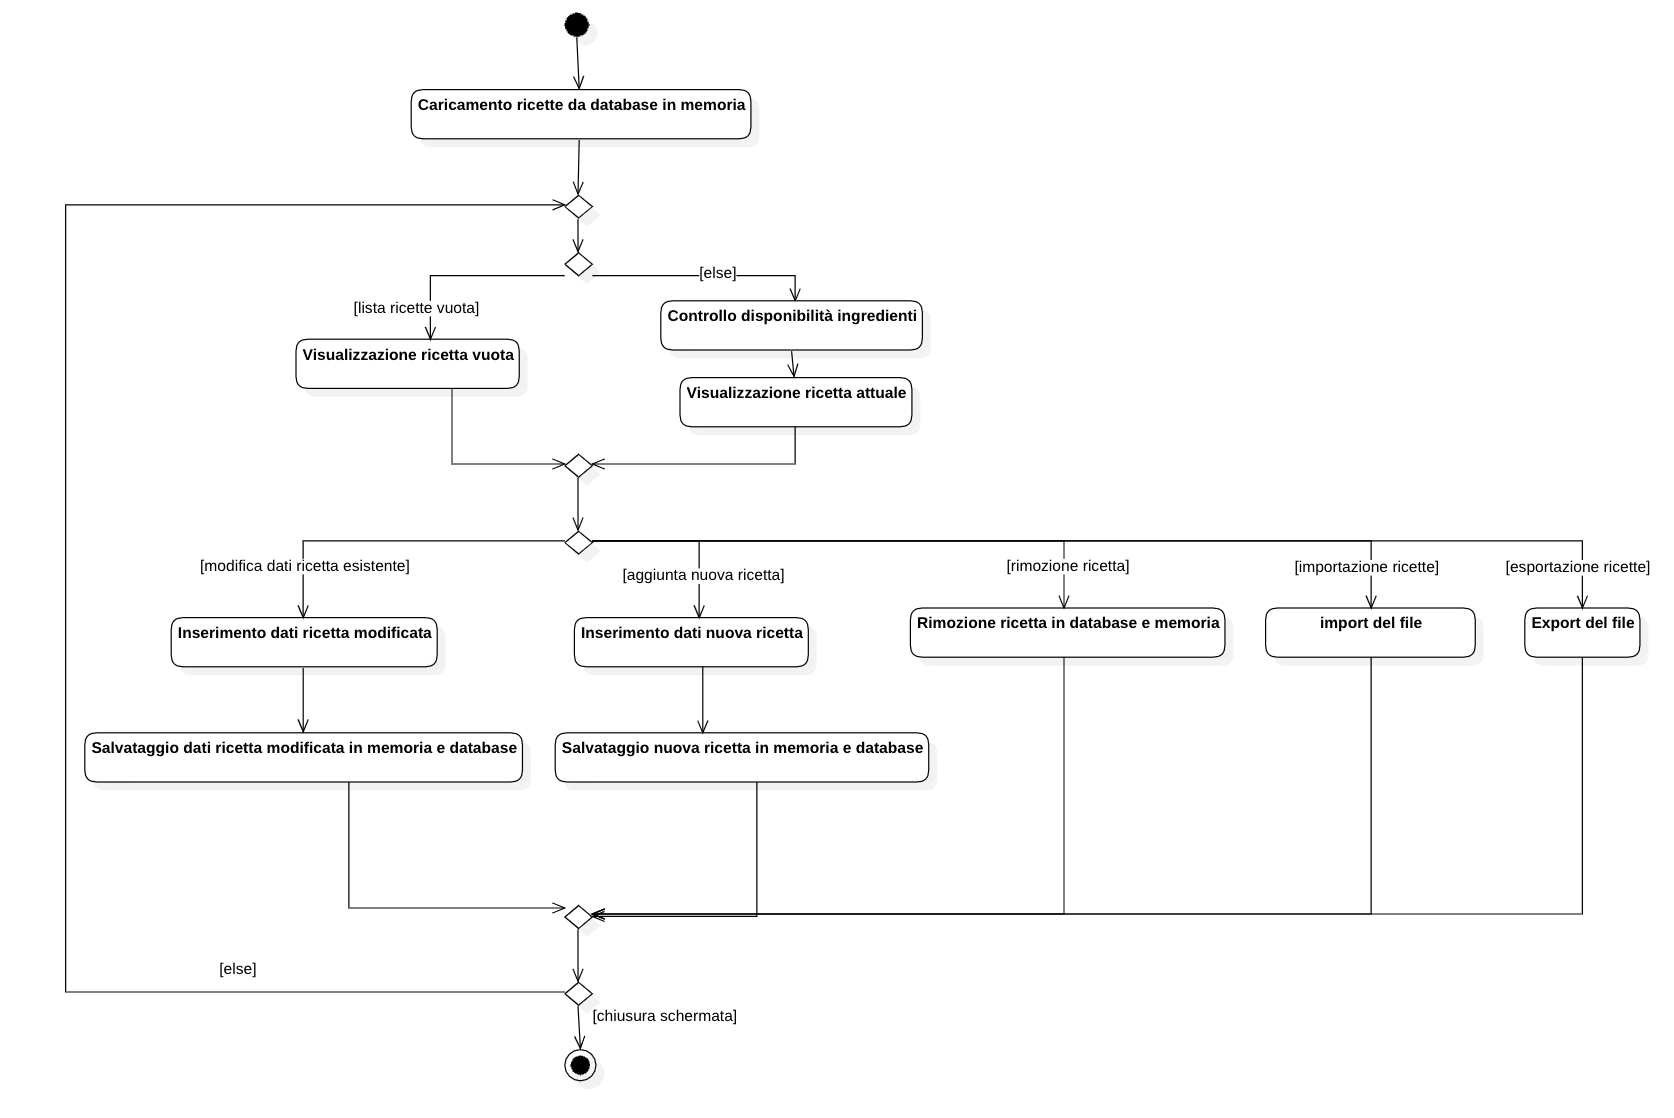
\includegraphics[width=\linewidth]{images/activity-recipe.png}
    \caption{Diagramma delle attività delle ricette.}
    \label{fig:actrecipe}
\end{figure}

\subsection{State diagram}

TODO.

\subsubsection{State diagram della ricetta}

TODO.

\begin{figure}[H]
    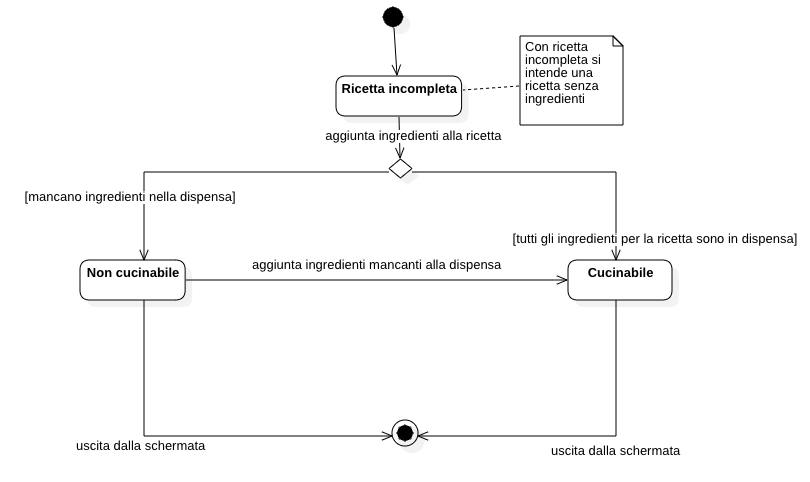
\includegraphics[width=\linewidth]{images/state-recipe.png}
    \caption{Diagramma degli stati della ricetta.}
    \label{fig:staterecipe}
\end{figure}

\subsubsection{State diagram della lista della spesa}

TODO.

\begin{figure}[H]
    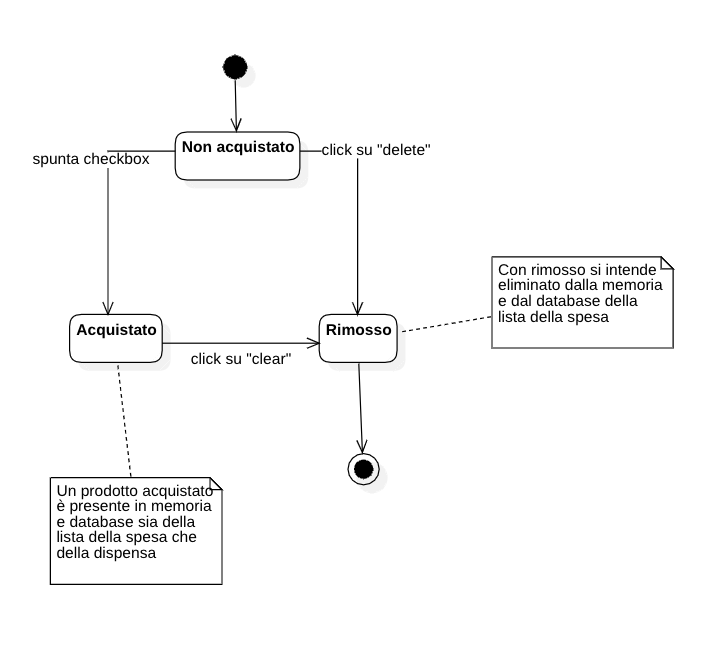
\includegraphics[width=\linewidth]{images/state-shopping-list.png}
    \caption{Diagramma degli stati della lista della spesa.}
    \label{fig:stateshoplist}
\end{figure}

\subsection{Class diagram}

TODO.

\begin{figure}[H]
    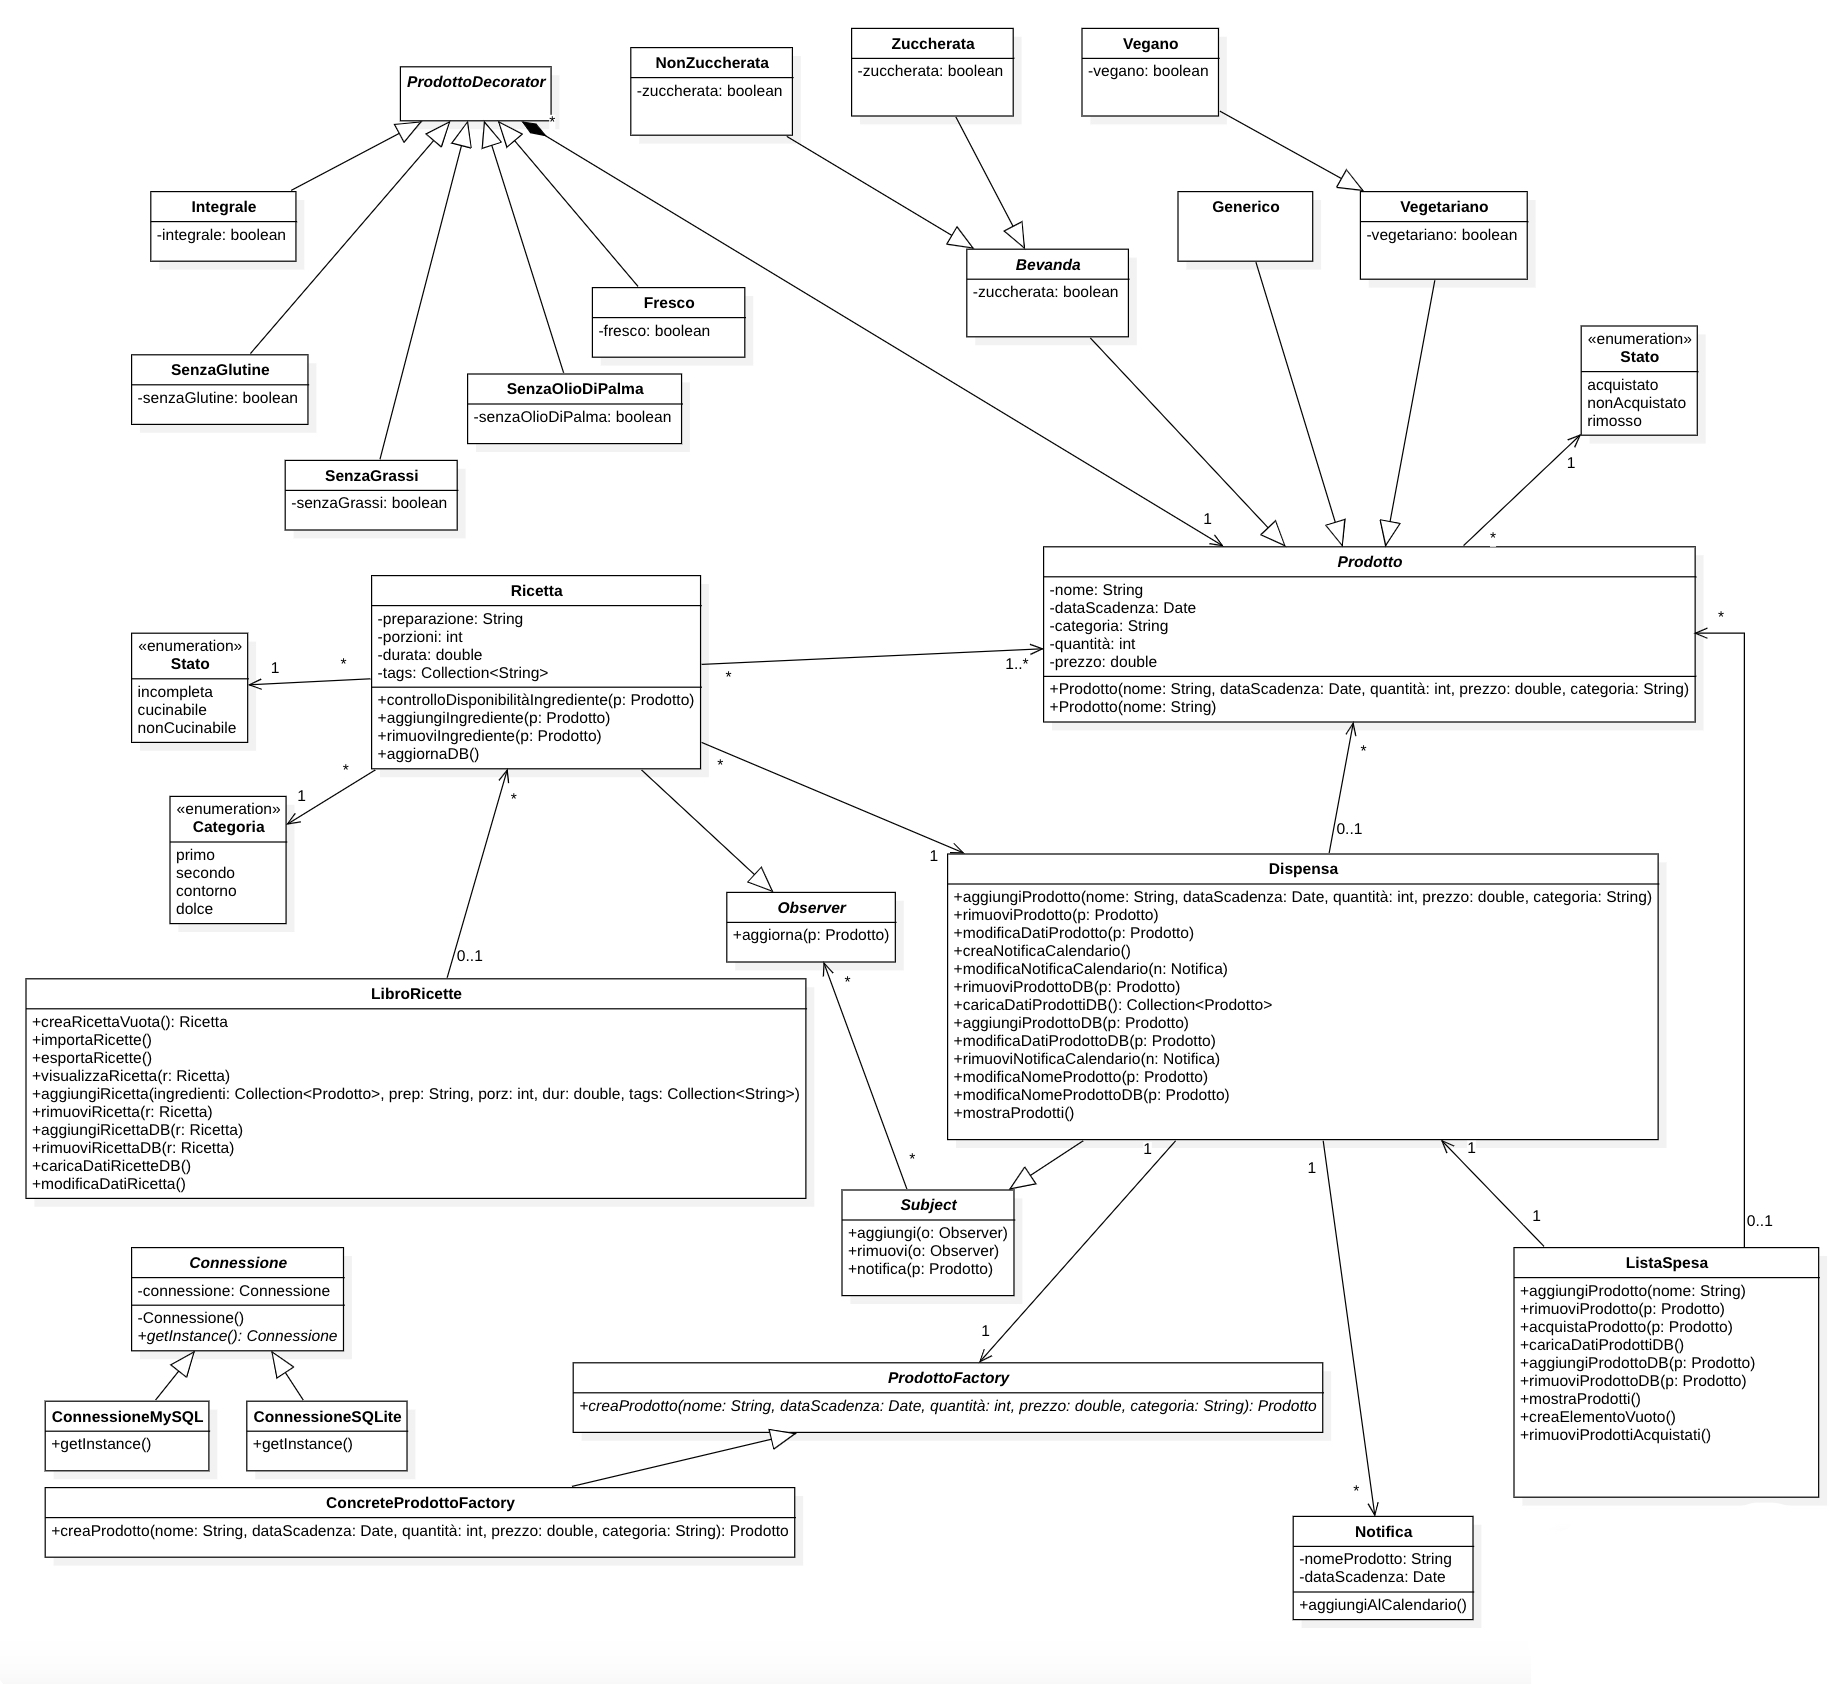
\includegraphics[width=\linewidth]{images/class.jpeg}
    \caption{Diagramma delle classi.}
    \label{fig:classdiagram}
\end{figure}

\subsection{Sequence diagram}

TODO.

\subsubsection{Sequence diagram della dispensa}

TODO.

\begin{figure}[H]
    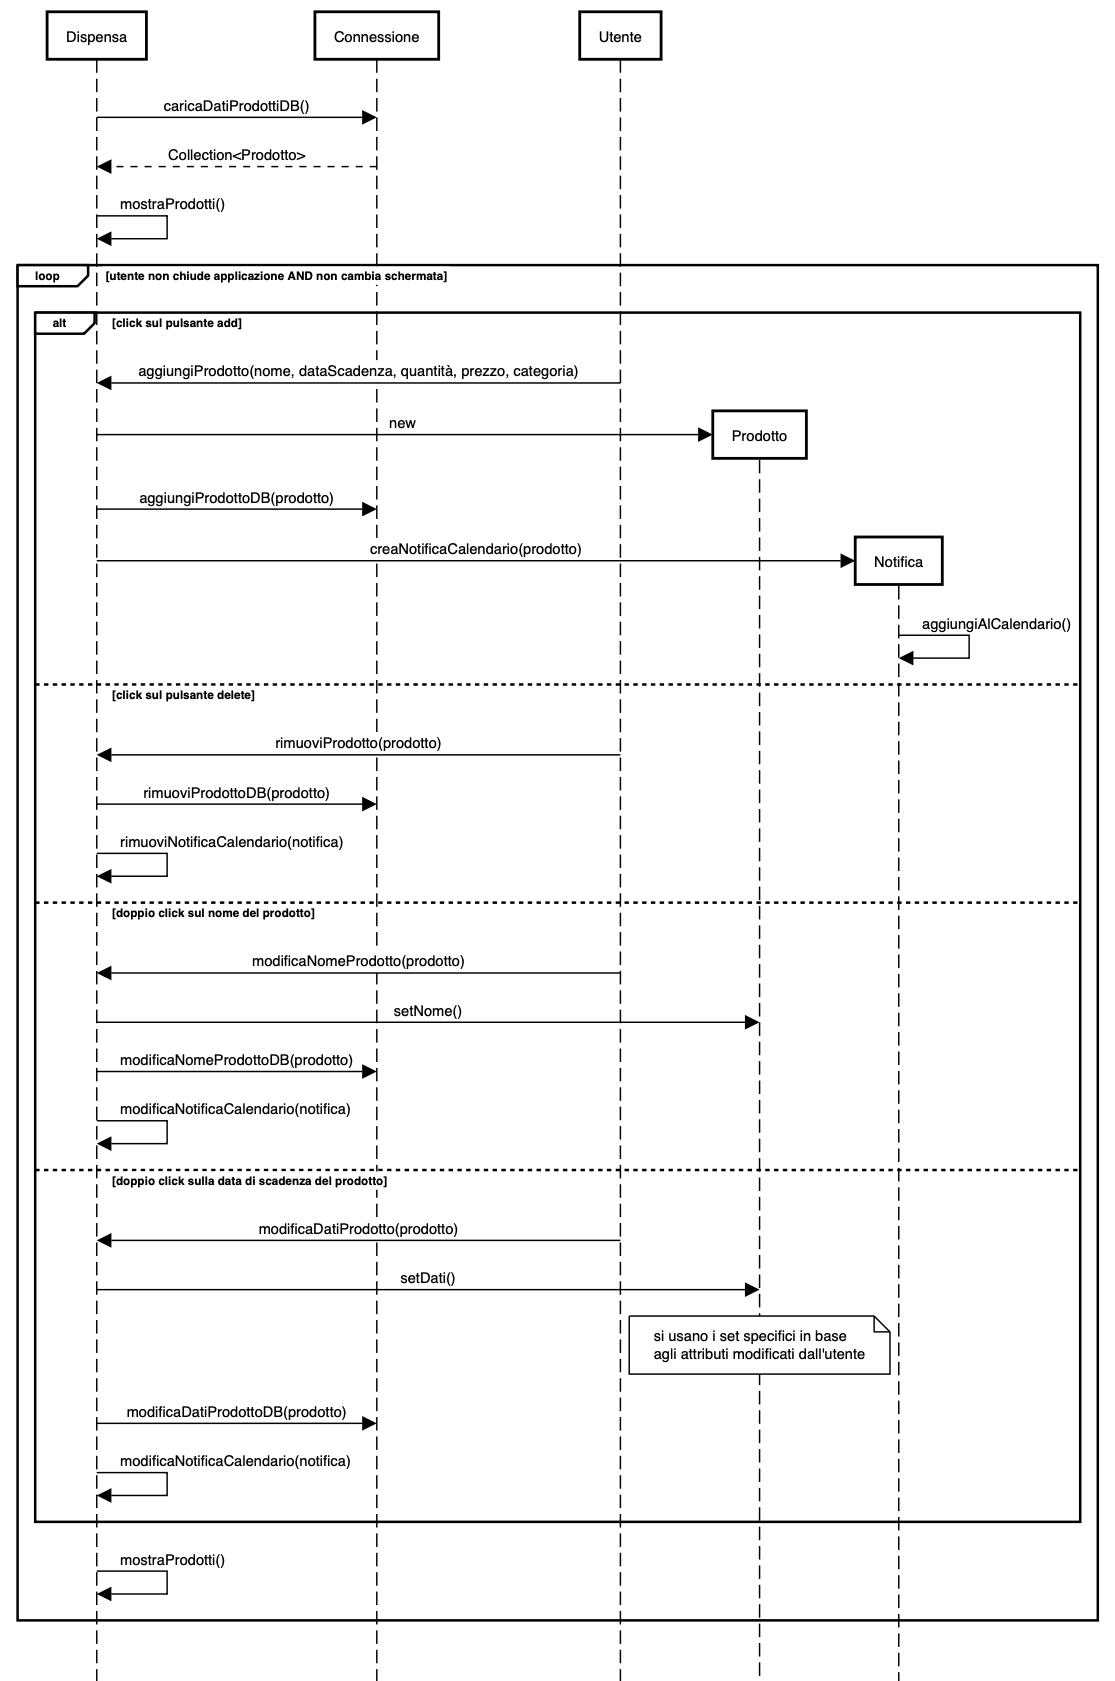
\includegraphics[width=\linewidth]{images/sequence-pantry.png}
    \caption{Diagramma di sequenza della dispensa}
    \label{fig:seqpantry}
\end{figure}

\subsubsection{Sequence diagram della lista della spesa}

TODO.

\begin{figure}[H]
    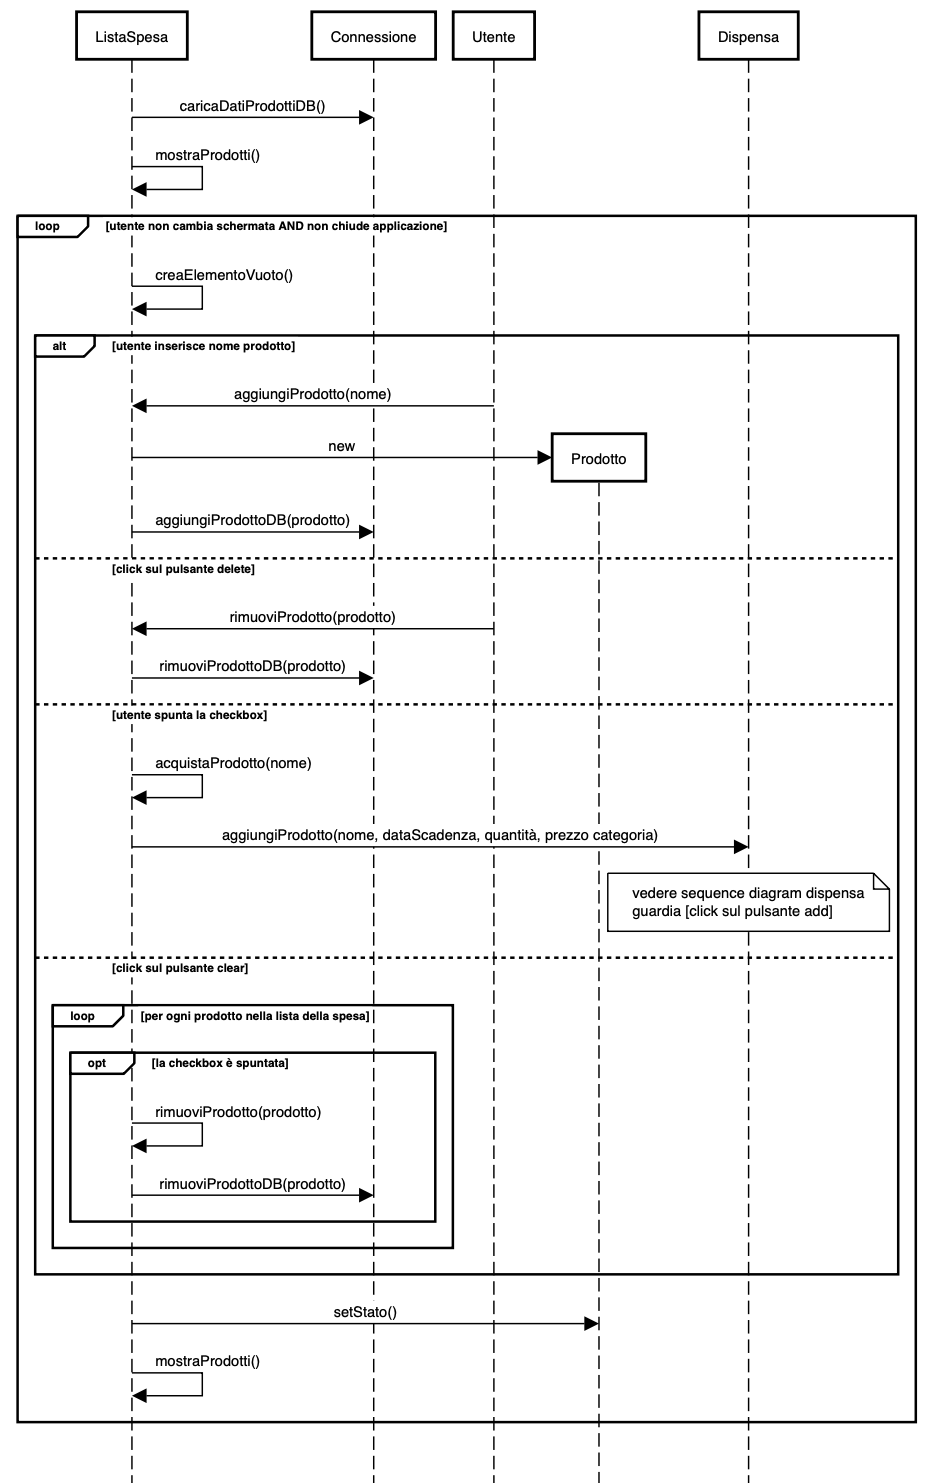
\includegraphics[width=\linewidth]{images/sequence-shopping-list.png}
    \caption{Diagramma di sequenza della lista della spesa}
    \label{fig:seqshoplist}
\end{figure}

\subsubsection{Sequence diagram delle ricette}

TODO.

\begin{figure}[H]
    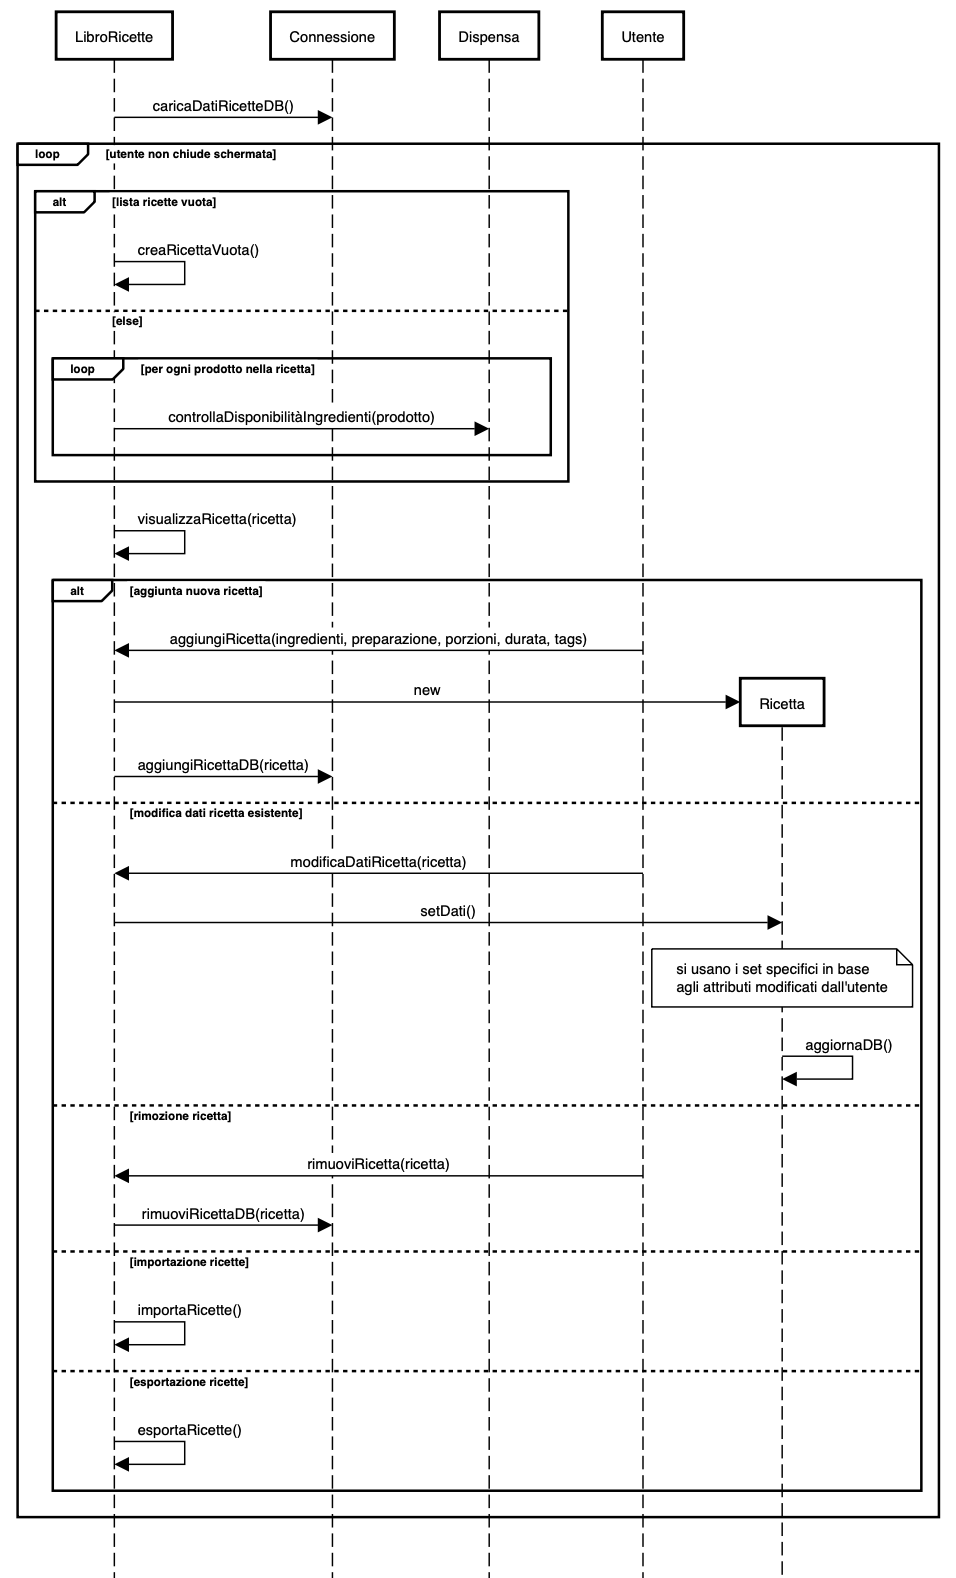
\includegraphics[width=\linewidth]{images/sequence-recipe.png}
    \caption{Diagramma di sequenza delle ricette}
    \label{fig:seqrecipe}
\end{figure}

\section{Design Pattern}

TODO.

\subsection{Factory}

TODO.

\subsection{Iterator}

TODO.

\subsection{Observer}

TODO.

\subsection{Singleton}

TODO.

\subsection{Decorator}

TODO.

\section{ORM}

TODO.

\subsection{Vantaggi}

TODO.

\subsection{Svantaggi}

TODO.

\subsection{Stress test}

TODO.

\end{document}